\documentclass[12pt]{article}

\usepackage{sbc-template}
\usepackage{graphicx,url}
\usepackage{float}
\usepackage[brazil]{babel}   
%\usepackage[latin1]{inputenc}  
\usepackage[utf8]{inputenc}  
\usepackage{url}

\usepackage{xcolor}
% Definindo novas cores
\definecolor{verde}{rgb}{0.25,0.5,0.35}
\definecolor{jpurple}{rgb}{0.5,0,0.35}
% Configurando layout para mostrar codigos Java
\usepackage{listings}

\bibliographystyle{ieeetr}

\definecolor{lightgray}{rgb}{.9,.9,.9}
\definecolor{darkgray}{rgb}{.4,.4,.4}
\definecolor{purple}{rgb}{0.65, 0.12, 0.82}

\lstdefinelanguage{JavaScript}{
	keywords={typeof, new, true, false, catch, function, return, null, catch, switch, var, if, in, while, do, else, case, break},
	keywordstyle=\color{blue}\bfseries,
	ndkeywords={class, export, boolean, throw, implements, import, this},
	ndkeywordstyle=\color{darkgray}\bfseries,
	identifierstyle=\color{black},
	sensitive=false,
	comment=[l]{//},
	morecomment=[s]{/*}{*/},
	commentstyle=\color{purple}\ttfamily,
	stringstyle=\color{red}\ttfamily,
	morestring=[b]',
	morestring=[b]"
}

\lstset{
	language=JavaScript,
	backgroundcolor=\color{lightgray},
	extendedchars=true,
	basicstyle=\footnotesize\ttfamily,
	showstringspaces=false,
	showspaces=false,
	numbers=left,
	numberstyle=\footnotesize,
	numbersep=9pt,
	tabsize=2,
	breaklines=true,
	showtabs=false,
	captionpos=b
}

\lstset{
	language=Java,
	basicstyle=\ttfamily\small, 
	keywordstyle=\color{jpurple}\bfseries,
	stringstyle=\color{red},
	commentstyle=\color{verde},
	morecomment=[s][\color{blue}]{/**}{*/},
	extendedchars=true, 
	showspaces=false, 
	showstringspaces=false, 
	numbers=left,
	numberstyle=\tiny,
	breaklines=true, 
	backgroundcolor=\color{cyan!10}, 
	breakautoindent=true, 
	captionpos=b,
	xleftmargin=0pt,
	tabsize=4
}
\pagestyle{empty}
     
\sloppy
	\title{Web Service de Consulta de CEP e Rastreamento de Encomendas dos Correios  \\ Exercício Computacional I - Sistemas Distribuídos}

\author{Rafael Gonçalves de Oliveira Viana\inst{1} \\\vspace*{10pt} \normalsize  \today{} }


\address{Sistemas de Informação -- Universidade Federal do Mato Grosso do Sul
	(UFMS)\\
  	Caixa Postal 79400-000 -- Coxim -- MS -- Brazil
  \email{rafael.viana@aluno.ufms.br}
}

\begin{document} 

\maketitle

     
\begin{resumo} 	
  Este relatório introduz a arquitetura de um \textit{Web Service} assim como seus componentes, o mesmo relata como foi implementado um Web Server que possui uma página web e um serviço para busca de CEP e rastreamento de encomendas dos Correios, utilizando Angular no \textit{front-end} e NodeJS no \textit{back-end}.
\end{resumo}



\section{Introdução}
  Com a diseminação de dispositivos com conexeção a Internet na sociedade atual, houvesse a necessidade de criar/gerenciar serviços web \textit{Web Services}, estes necessarios para atender as mais diversas funções como o rastreio de encomendas e consultas de CEPs entre outros serviços.
  Este relatório demonstrará  a arquitetura de um \textit{Web Service} e como foi implementado um \textit{Web Service} de consulta de CEP e rastreamento de encomendas dos correios, juntamente com uma página web que consome os serviços.
  O código deste relatório esta em sua totalidade no endereço http://github.com/rafaelgov95/SD/Projeto-Correios-Angular2, e o mesmo pode ser reutilizado sobre a licença MIT.
\section{Arquitetura de um Web Service}
Para poder identificar qual arquitetura que um \textit{Web Service} deve possuir devemos examinar os papéis individuais de cada ator no \textit{Web Service} e examinar a pilha emergente de protocolo que o mesmo pretende utiliza.
O mesmo pode ser publicado na intranet ou na Internet, provendo três possiveis formatos de serviços: Provedor de Serviço, Solicitante de Serviço e o Registro de Serviço.
Para mais detalhes desta sessão incentivo consultar \cite{tutorial}. 

\begin{enumerate}
	\item \textbf{Provedor de serviço:}
	Fornece serviços web. O provedor de serviços implementa o serviço e disponibiliza-o na Internet ou intranet.
	\item \textbf{Solicitante de Serviço:}
	Este é um consumidor do serviço web. O solicitante utiliza um serviço da Web existente abrindo uma conexão de rede e enviando uma solicitação XML.
	\item \textbf{Registro de serviço:}
	Este é um diretório de serviços logicamente centralizado. O registro fornece um lugar central onde os desenvolvedores podem publicar novos serviços ou encontrar os existentes. Ele serve como centro de compensação centralizado para empresas e seus serviços.
\end{enumerate}


\subsection{Pilha de protocolo de um \textit{Web Service}}
Uma segunda opção para identificar qual arquitetura o  \textit{Web Service} deve utiliza é examinar a pilha emergente de protocolo que pretende utilizar. Cada dia existe mais tipos de protocolos porém existem 4 tipo que se destacam: Serviço de Transporte - "FTP", Mensagens "XML", Descrição de Serviço "WSDL"  e Descoberta de Serviço "UDDI" 
\begin{enumerate}
	\item \textbf{Serviço de transporte:}
	Esta camada é responsável pelo transporte de mensagens entre aplicativos. Atualmente, esta camada inclui o protocolo de transporte de hipertexto (HTTP), protocolo de transferência de correio simples (SMTP), protocolo de transferência de arquivos (FTP) e protocolos mais recentes, como o protocolo de intercâmbio extensível de blocos (BEEP).
	\item \textbf{Mensagens XML:}
	Esta camada é responsável por codificar mensagens em um formato XML comum para que as mensagens possam ser entendidas em cada uma das extremidades. Atualmente, esta camada inclui XML-RPC e SOAP.
	\item \textbf{Descrição do Serviço:}
	Esta camada é responsável por descrever a interface pública para um serviço web específico. Atualmente, a descrição do serviço é tratada através do Web Service Description Language (WSDL).

	\item \textbf{Descoberta do serviço:}
	Esta camada é responsável por centralizar os serviços em um registro comum e fornecer funcionalidades fáceis de publicação / pesquisa. Atualmente, a descoberta do serviço é tratada através de Descrição Universal, Descoberta e Integração (UDDI).
\end{enumerate}

\subsection {Principais Serviço de Transporte de um Web Service}Os protocolos da camada inferior ficam respornsaveis pelo transporte de serviços. Essa camada é responsável por transportar como exemplo mensagens XML e JSON entre dois computadores.
\begin{enumerate}
	\item \textbf{Hyper Text Transfer Protocol (HTTP):}
	É a opção mais popular para o transporte de serviços. O HTTP é simples, estável e amplamente implantado. Além disso, a maioria dos firewalls permitem o tráfego HTTP. Isso permite que mensagens REST ou SOAP se mostrem como mensagens HTTP. Isso é bom se você quiser integrar aplicativos remotos, mas eleva uma série de preocupações de segurança.
	\item \textbf{Bloqueia o protocolo de troca extensível (BEEP)}
	Esta é uma alternativa promissora para o HTTP. O BEEP é uma nova estrutura da Task Force de Engenharia da Internet (IETF) para a construção de novos protocolos. O BEEP está em camadas diretamente no TCP e inclui uma série de recursos internos, incluindo um protocolo inicial de handshake, autenticação, segurança e tratamento de erros. Usando BEEP, pode-se criar novos protocolos para uma variedade de aplicações, incluindo mensagens instantâneas, transferência de arquivos, distribuição de conteúdo e gerenciamento de rede.
	O SOAP não está vinculado a nenhum protocolo de transporte específico. Na verdade, você pode usar SOAP via HTTP, SMTP ou FTP. Uma idéia promissora é, portanto, usar SOAP sobre BEEP.
\end{enumerate}
\begin{figure}[H]
	\centering
	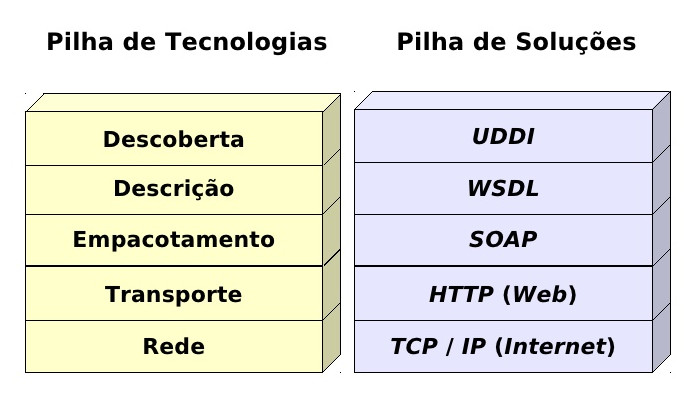
\includegraphics[scale=0.5]{Imagens/pilhat.jpg}
	\caption{Pilha de protocolo de transporte e suas tecnologias. }
	\label{wbs}
\end{figure}


\subsection{Componentes de um \textit{Web Service}}
Ao longo dos últimos anos, três tecnologias primárias emergiram como padrões mundiais que constituem o núcleo da tecnologia de serviços da Web de hoje. Essas tecnologias são demostradas abaixo.


\subsubsection{WSDL - \textit{Web Services Description Language} }
O WSDL é um idioma baseado em XML para descrever os serviços da Web e como acessá-los.

\begin{enumerate}
	\item O WSDL foi desenvolvido conjuntamente pela Microsoft e pela IBM.
	\item WSDL é um protocolo baseado em XML para troca de informações em ambientes descentralizados e distribuídos.
	\item WSDL é o formato padrão para descrever um serviço web.
	\item A definição WSDL descreve como acessar um serviço da Web e quais as operações que ele executará.
	\item O WSDL descrever como se relacionar com serviços baseados em XML.
	\item WSDL é parte integrante do UDDI, um registro de negócios mundial baseado em XML.
	\item WSDL é o idioma que UDDI usa.
	
\end{enumerate}

\subsubsection{SOAP - \textit{Simple Object Access Protocol}}
O SOAP é um protocolo baseado em XML para trocar informações entre computadores.

\begin{enumerate}
	\item O SOAP será desenvolvido como um padrão W3C.
	\item O SOAP é um protocolo de comunicação.
	\item O SOAP é para comunicação entre aplicativos.
	\item O SOAP é um formato para enviar mensagens.
	\item O SOAP é projetado para se comunicar via Internet.
	\item O SOAP é independente da plataforma.
	\item O SOAP é independente da linguagem.
	\item O SOAP é simples e extensível.
	\item O SOAP permite que você percorra os firewalls.
\end{enumerate}
\subsubsection{REST - \textit{Representation State Transfer}}
É uma arquitetura criada para ser mais simples de se usar que o SOAP. Este pode ser usado em vários formatos de texto, como CSV (Comma-separated Values), RSS (Really Simple Syndication), JSON e YAML. Porém, só pode ser utilizado com o protocolo HTTP/HTTPS, por exemplo utilizando os métodos GET, POST, PUT e DELETE. 

\begin{enumerate}
	\item Melhor curva de aprendizado.
	\item Mensagens menores e mais eficientes como o formato JSON comparado com XML.
	\item Os dados podem ser colocados em cache, retornando sempre a mesma resposta para a mesma requisição.
	\item Mais rápido pois precisa de menos processamento que o SOAP.
\end{enumerate}
\subsection{Exemplo Ilustrativo de um Web Service}
\begin{figure}[H]
	\centering
	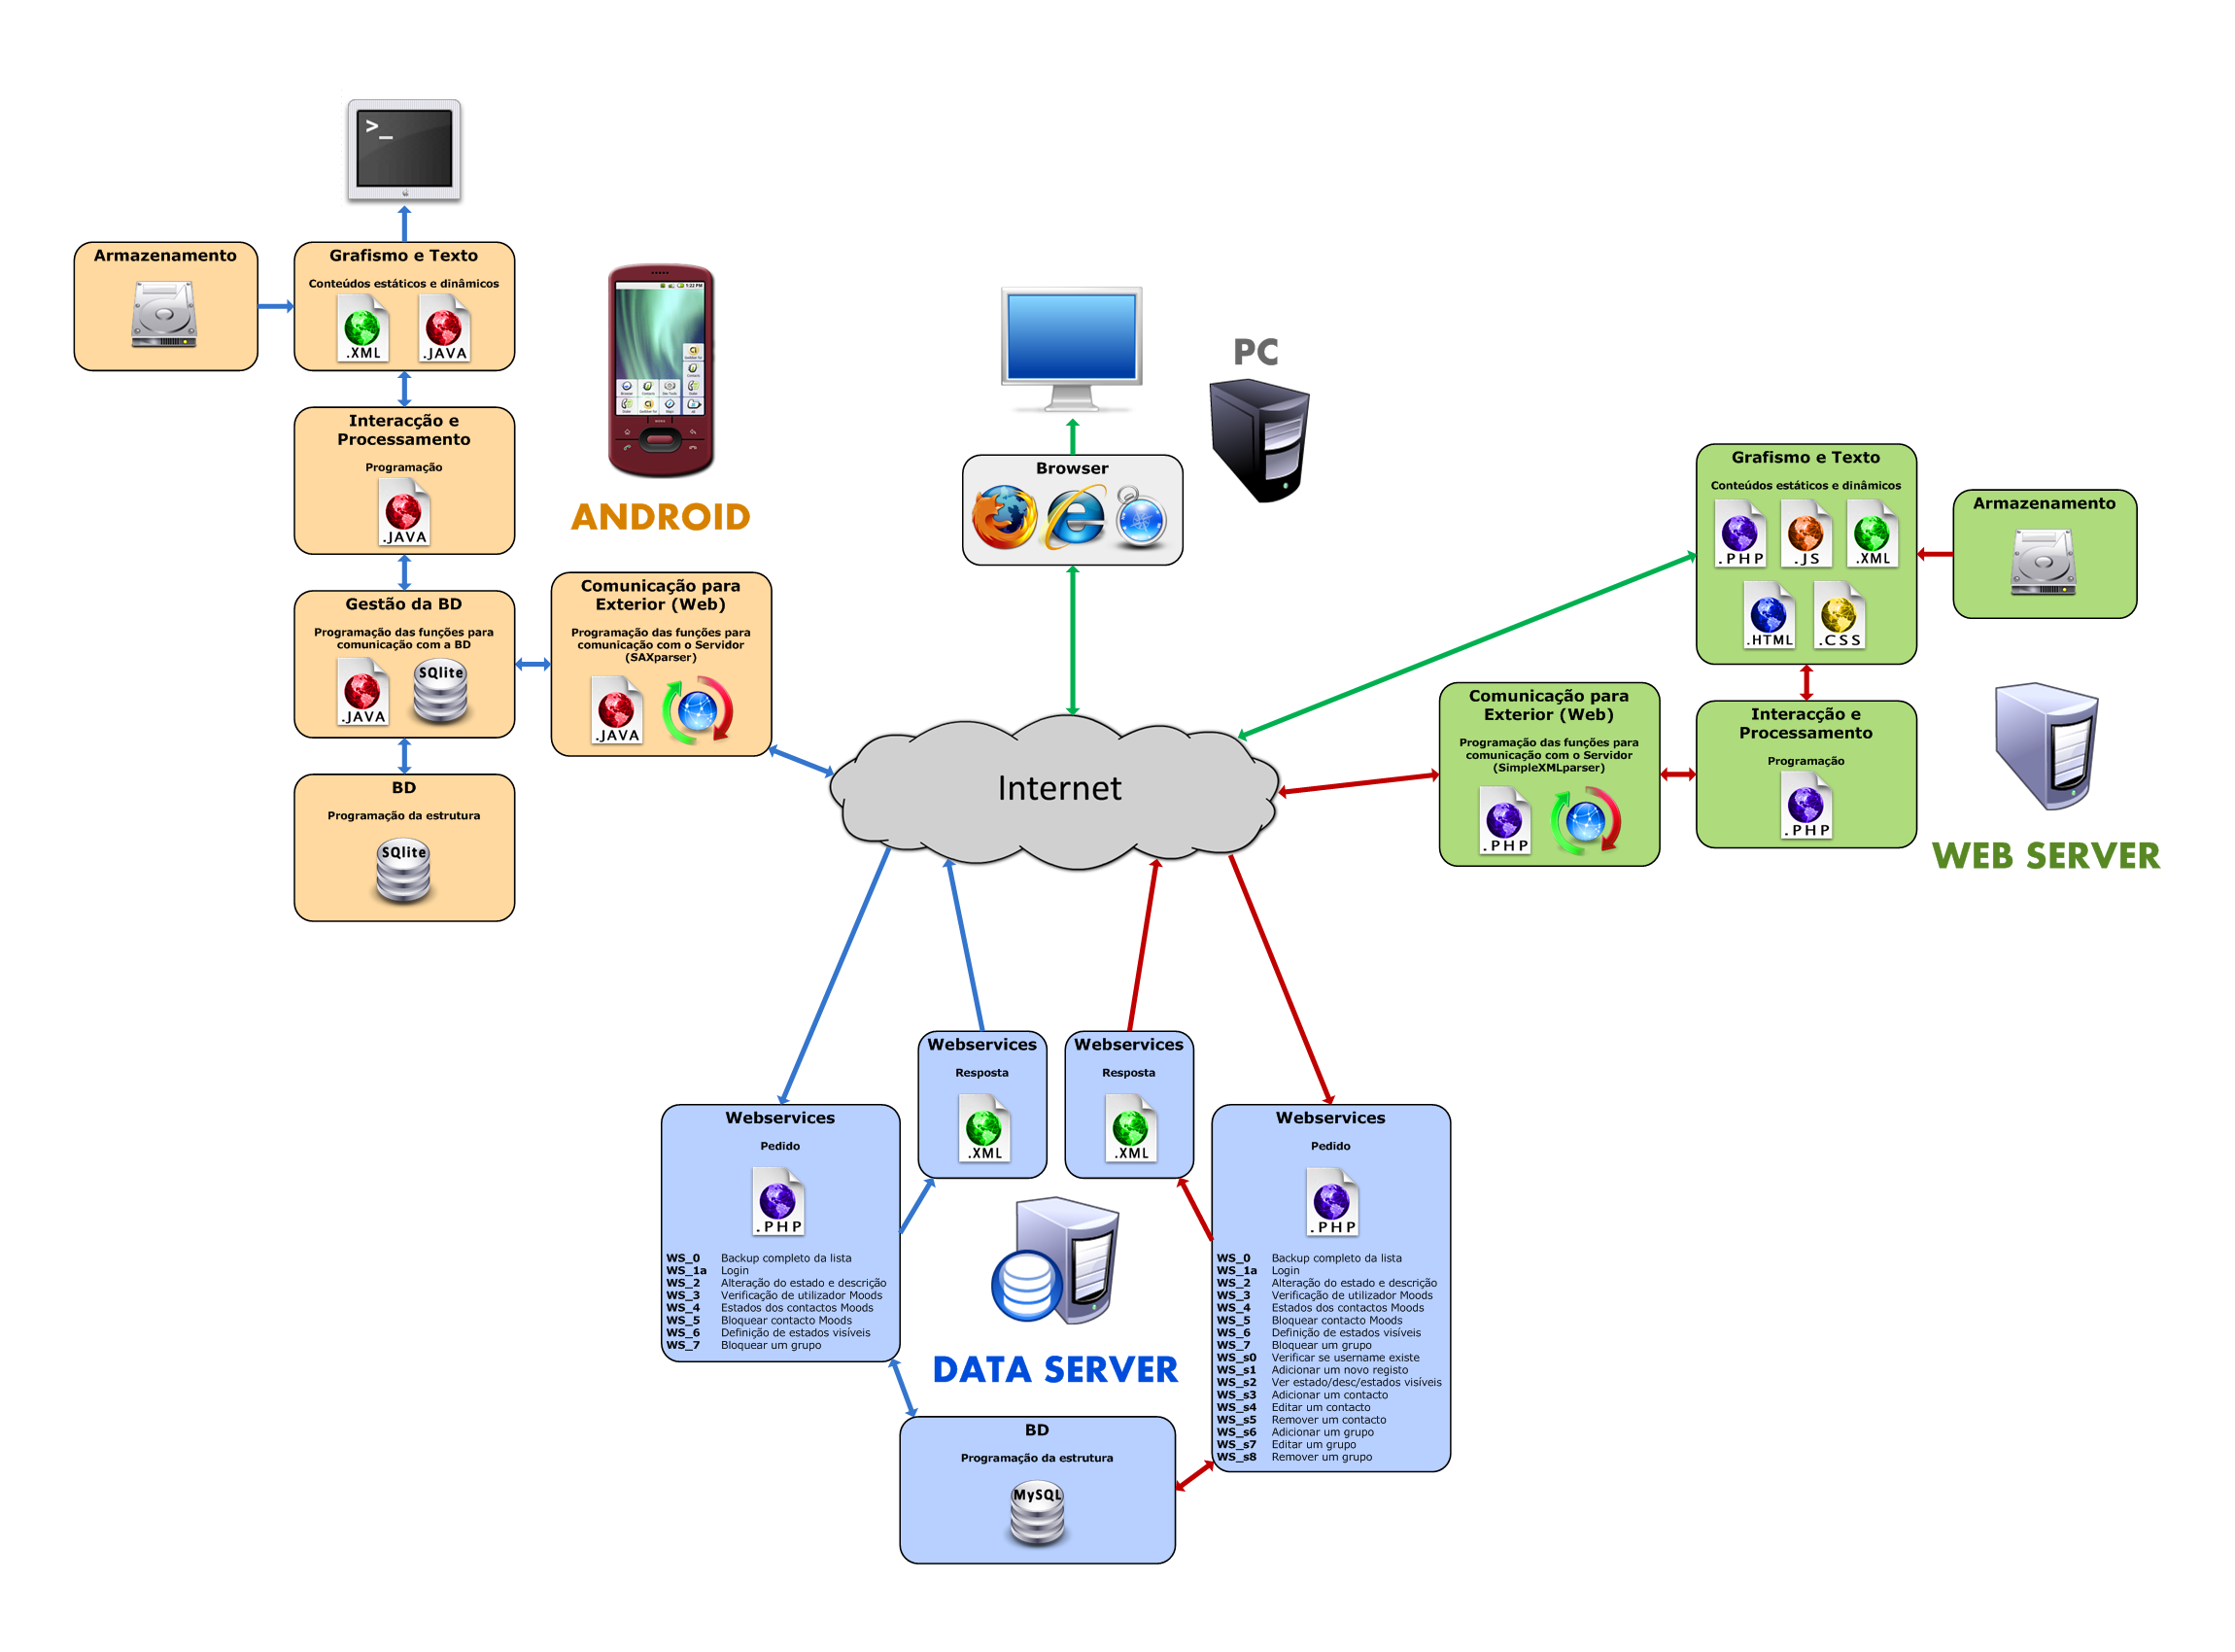
\includegraphics[scale=0.18]{Imagens/webservice.png}
	\caption{Sistema implantando fornecendo serviços para diversos sistemas clientes diferentes.}
	\label{wbs}
\end{figure}
\section{Metodologia}
Nesta sessão será relatado como foi o desenvolvimento e a implantação de um \textit{Web Service} em um \textit{Web Server} que realiza busca de CEPs e rastreamento de encomendas dos correios.
 
\subsection{Web Server}
	O \textit{Web Server} foi implementado utilizando o NodeJS com o framework ExpressJs, onde cria um ambiente de desenvolvimento para criação de Web Services.
	\begin{quote}
	O Node.js usa um modelo de E/S não bloqueante, que o torna leve e eficiente. O ecossistema de pacotes Node.js, npm , é o maior ecossistema de bibliotecas de código aberto do mundo \cite{nodejs}.
	\end{quote}
	\begin{quote}
	O Express é um framework para aplicativo da web do Node.js mínimo e flexível que fornece um conjunto robusto de recursos para aplicativos web e móvel \cite{expressjs}.
	\end{quote}

\subsection{Web Service de Busca de CEP}
	A busca de ceps esta sendo tercerizada por um \textit{Web Service} que prove consultas de CEPs, nos mais diversos tipos de empacotamento. Esses serviços são fornecidos pela impresa	\textit{VIACEP}, o site da mesma é https://viacep.com.br/.

	Uma página Web RafaelBuscas foi construida utilizando o framework Angular, a mesma consome o serviço de buscas de cep, no formato JSON fornecido pelos servidores da Viacep.
	
	A url do Web Service da VIACEP, consumido pela página RafaelBuscas, foi o http://viacep.com.br/ws/01001000/json/, o mesmo retorna uma resposta em JSON, com as informações do CEP (Localização, Bairro, Código IBGE, GIA), para mais informações sobre requisições consultar \cite{viacep}. 
	
\subsection{Web Service Encomendas dos Correios}
	O rastreiamento por encomendas dos correios foi feita com duas tecnologias diferentes de empacontamento, fornecidos pelos Servidores dos Correios, um utiliza a tecnologia SOAP e outra alternativa e utilizar um requisição REST HTTP-POST e parsear a resposta de uma página HTML, cada uma das opções serão discutidas abaixo.
\subsubsection{Serviço de Rastreamento Encomenda via SOAP}
O WSDL dos correios que fornece recursos para os serviços de requisição SOAP. 

O Serviço de Rastreamento de Encomendas dos correios via SOAP é gratuito.

A Url "http://webservice.correios.com.br:80/service/rastro" é o endereço do \textit{Web Service} e não do wsdl, o webservice espera uma mensagem SOAP como na Listing \ref{c1} a mesma deve ser assinada com cabeçalhos HTTP no formato "Content-Type", "text/xml".
\lstset{
	language=xml,
	tabsize=3,
	%frame=lines,
	caption=Código XML SOAP para requisição de localização de pacote,
	label=c1,
	frame=shadowbox,
	rulesepcolor=\color{gray},
	xleftmargin=20pt,
	framexleftmargin=15pt,
	keywordstyle=\color{blue}\bf,
	commentstyle=\color{OliveGreen},
	stringstyle=\color{red},
	numbers=left,
	numberstyle=\tiny,
	numbersep=5pt,
	breaklines=true,
	showstringspaces=false,
	basicstyle=\footnotesize,
	emph={food,name,price},emphstyle={\color{magenta}}}
\lstinputlisting{Codigo/codigo1.xml}

Utilizando a linguagem Java e a biblioteca \textit{javax.xml.soap} foi feita uma simulação de envio de requisição SOAP com a mensagem Listing \ref{c1} para o \textit{Web Service} de rastreamento de encomendas, fornecido pelos correios para mais informações encentivo consultar \cite{correios}.

O retorno da requisição é um código XML contendo a resposta da requsição, como demostrano na Listing \ref{c2}.
 \lstset{
 	language=xml,
 	tabsize=3,
 	%frame=lines,
 	caption=Resposta da Requisição SOAP,
 	label=c2,
 	frame=shadowbox,
 	rulesepcolor=\color{gray},
 	xleftmargin=20pt,
 	framexleftmargin=15pt,
 	keywordstyle=\color{blue}\bf,
 	commentstyle=\color{OliveGreen},
 	stringstyle=\color{red},
 	numbers=left,
 	numberstyle=\tiny,
 	numbersep=5pt,
 	breaklines=true,
 	showstringspaces=false,
 	basicstyle=\footnotesize,
 	emph={food,name,price},emphstyle={\color{magenta}}}
 \lstinputlisting{Codigo/codigo2.xml}
 Esse serviço disponibilizado pelos correios apesar de ser gratuito somente retorna a última atualização do objeto, como demostrado na Listing \ref{c2}.
\subsubsection{Serviço de Rastreamento de Encomendas alternativo utilizando Crawling na Página dos Correios}

	Existe um serviço disponível na página dos correios para rastreamento de encomendas utilizando esse serviço da página web é possivel fazer um Crawling da página, com o objetivo de extrair as informações da encomenda.
	
	O serviço está disponível na url "http://www2.correios.com.br/sistemas/rastreamento/", a imagem \ref{c1} demostra como pode-se utilizando a ferramenta \textit{Postman} para realizar uma requsição Rest HTTP-POST, direto para página de rastreamento com objetivo de extrair informações da mesma.
	
	 \begin{figure}[H]
	 	\centering
	 	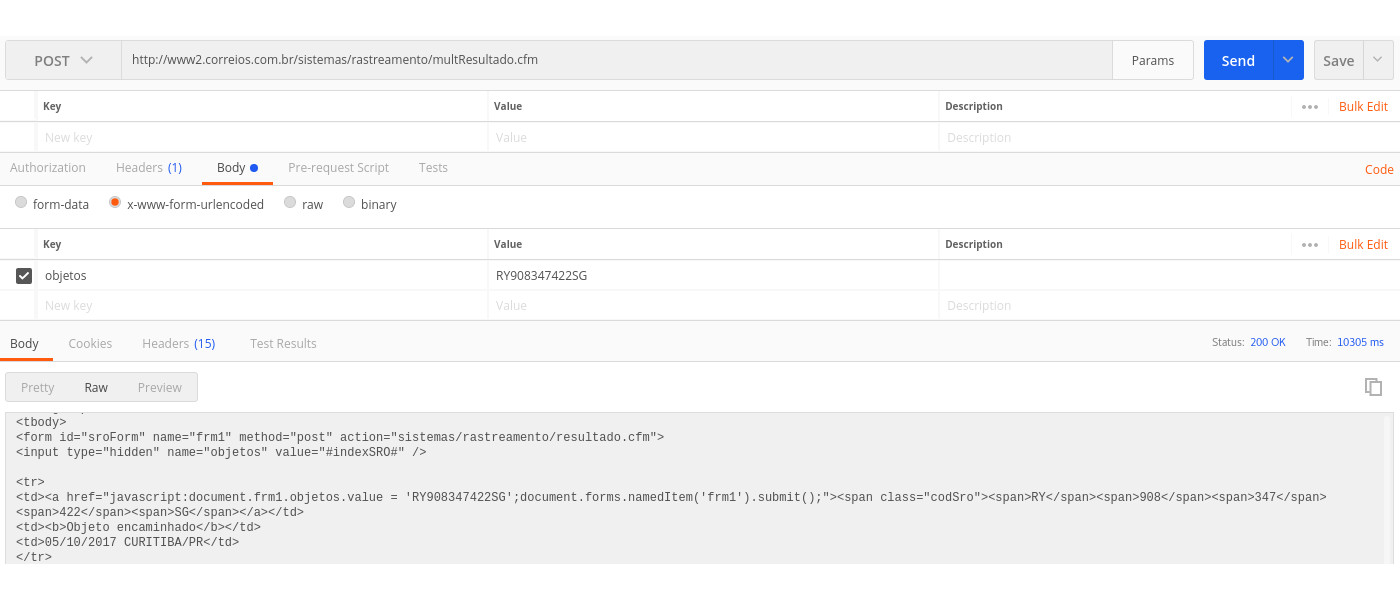
\includegraphics[scale=0.3]{Imagens/c1.jpg}
	 	\caption{Postman realizando um requsição REST HTTP-POST.}
	 	\label{c1}
	 \end{figure}
	
	Para consumir o serviço da página dos correios primeiramente temos que criar um \textit{Web Service} com NodeJs e o framework ExpressJs, junto com a biblioteca request-promise para requisição JavaScript e a biblioteca cheerio para realizar o parse das tag do HTML.
	
	Na Listing \ref{c3} foi criado um método que realiza um requisição REST - HTTP-POST no \textit{Web Server} da página web.
	
	\medskip
	\begin{lstlisting}[caption=Criando Requisição em Java Script,label=c3]
	request: function (req) {
	var correios = {
	uri: "http://www2.correios.com.br/sistemas/rastreamento/multResultado.cfm",
	form: {
	objetos: req.params.code
	},
	method: 'POST',
	headers: {}
	};
		response = requestPromise(correios);
		console.log(response)
		return response
	}	
	\end{lstlisting}
	Após a requsição da  Listing \ref{c3}, um variável data contendo todo o HTML da requsição e parseado pela função na Listing \ref{c4}, com o objetivo de extrair as informações necessárias.
	
	O parse percorre a tabela e extrai, algumas informações (código, localidade, data, situação) com objetivo de criar um objeto JSON, com as informações de rastreamento que será consumido pela página web (RafaelBuscas).
	
	Sendo assim uma requisição através da página RafaelBuscas ou utilizando diretamente a url http://rafaelbuscas.ddns.bet/json/"codigo-de-rastreamento", primeiramente e recebida pelo \textit{Web Service} que está aguardando na rota da url acima, após recebido uma requisição o mesmo requisita a página de rastreamento dos correios com o código fornecido, e depois realiza um parse da página extraindo as informações e encaminhando o objeto em JSON como response para requisição inicial.   
	\medskip
	\begin{lstlisting}[caption=Criando um Crawling para parsar as tags,label=c4]
	
	parser: function (data) {
		var $ = cheerio.load(data);
		var objetos = [];
		var tableObjetos = $('table').find('tr');
		$(tableObjetos).map(function(key, objeto){
			objeto  = $(objeto).children('td').map(function (key, field) {
				return $(field).text();
			}).toArray();
			if (objeto[0]) {
				
				var rastreio = {
					codigo  : null,
					situacao: null,
					local   : null,
					data    : null
				};
				
				rastreio.codigo     = objeto[0].trim();
				if (objeto[2]) {
					rastreio.situacao   = objeto[1];
					rastreio.local      = objeto[2].substr(11, objeto[2].length).trim();
					rastreio.data       = objeto[2].substr(0,10).trim();
				} else {
					rastreio.situacao   = 'Objeto ainda nao consta no sistema'
				}
				
				objetos['rast'] = rastreio;
			}
		});
		
		return Object.assign({}, objetos);
	}
	  	\end{lstlisting}
	  	
	  	
	  	\section{Página RafaelBuscas}
	  	Para fins didaticos os serviços criados nesse relatório estão disponíveis na url http://rafaelbuscas.ddns.net.
	  	
	  	Essa página está hospedada em uma máquina virtual do Google Cloud, a mesma está disponível para buscas de cep e rastreamento de encomendas sem custos.
	  	Na página inical no canto inferior tem um input para colocar o código do CEP ou do Rastreamento, um componente para seleção de Cep ou Rastremamento com nome de TIPO, tem que ser marcado como CEP ou Rastreio, antes da busca(butão com uma lupa) como demostrado na Figura \ref{c2}.
	  	
	  		 \begin{figure}[H]
	  		\centering
	  		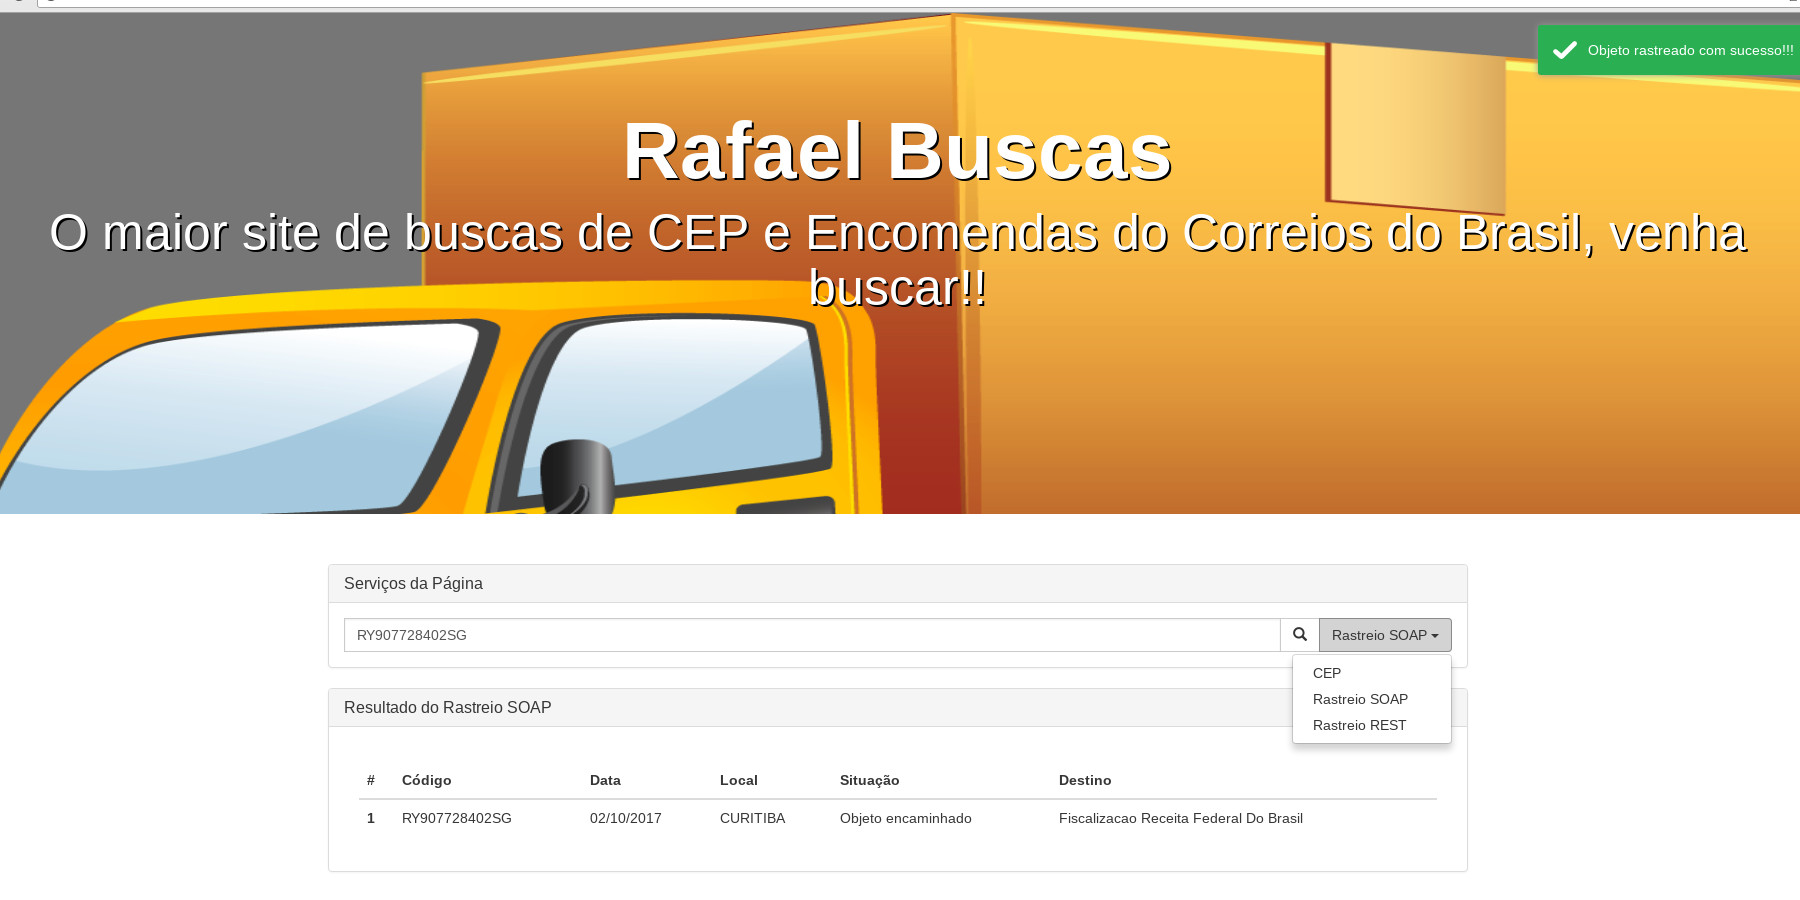
\includegraphics[scale=0.23]{Imagens/c2.jpg}
	  		\caption{Página RafaelBuscas, demostração de busca de cep.}
	  		\label{c2}
	  	\end{figure}
\section{Conclusão}
Esse relatório demostro como pode ser criado uma página web e um \textit{web service}  que consome serviços de outros \textit{Web Services} disponíveis por outras impresas, ou utilizar os mesmos para criação de um novo serviço, para atender as mais diversas necessidades.	  	

	  \bibliography{bibli}

\end{document}


